\documentclass[../delivery_hospital_report.tex]{subfiles}
\graphicspath{ {images/}{../images/}{../../images/} }
\begin{document}

\section{Sinalização}
\subsection{Placa}
%================================ SINALIZAÇÂO PROTÒTIPO========================
\subsubsection{Protótipo}

\paragraph{Esquemático}

\begin{figure}[h]
\centering
    \caption{Protótipo placa de Sinalização - Esquemático principal }
    \centering % para centralizarmos a figura
    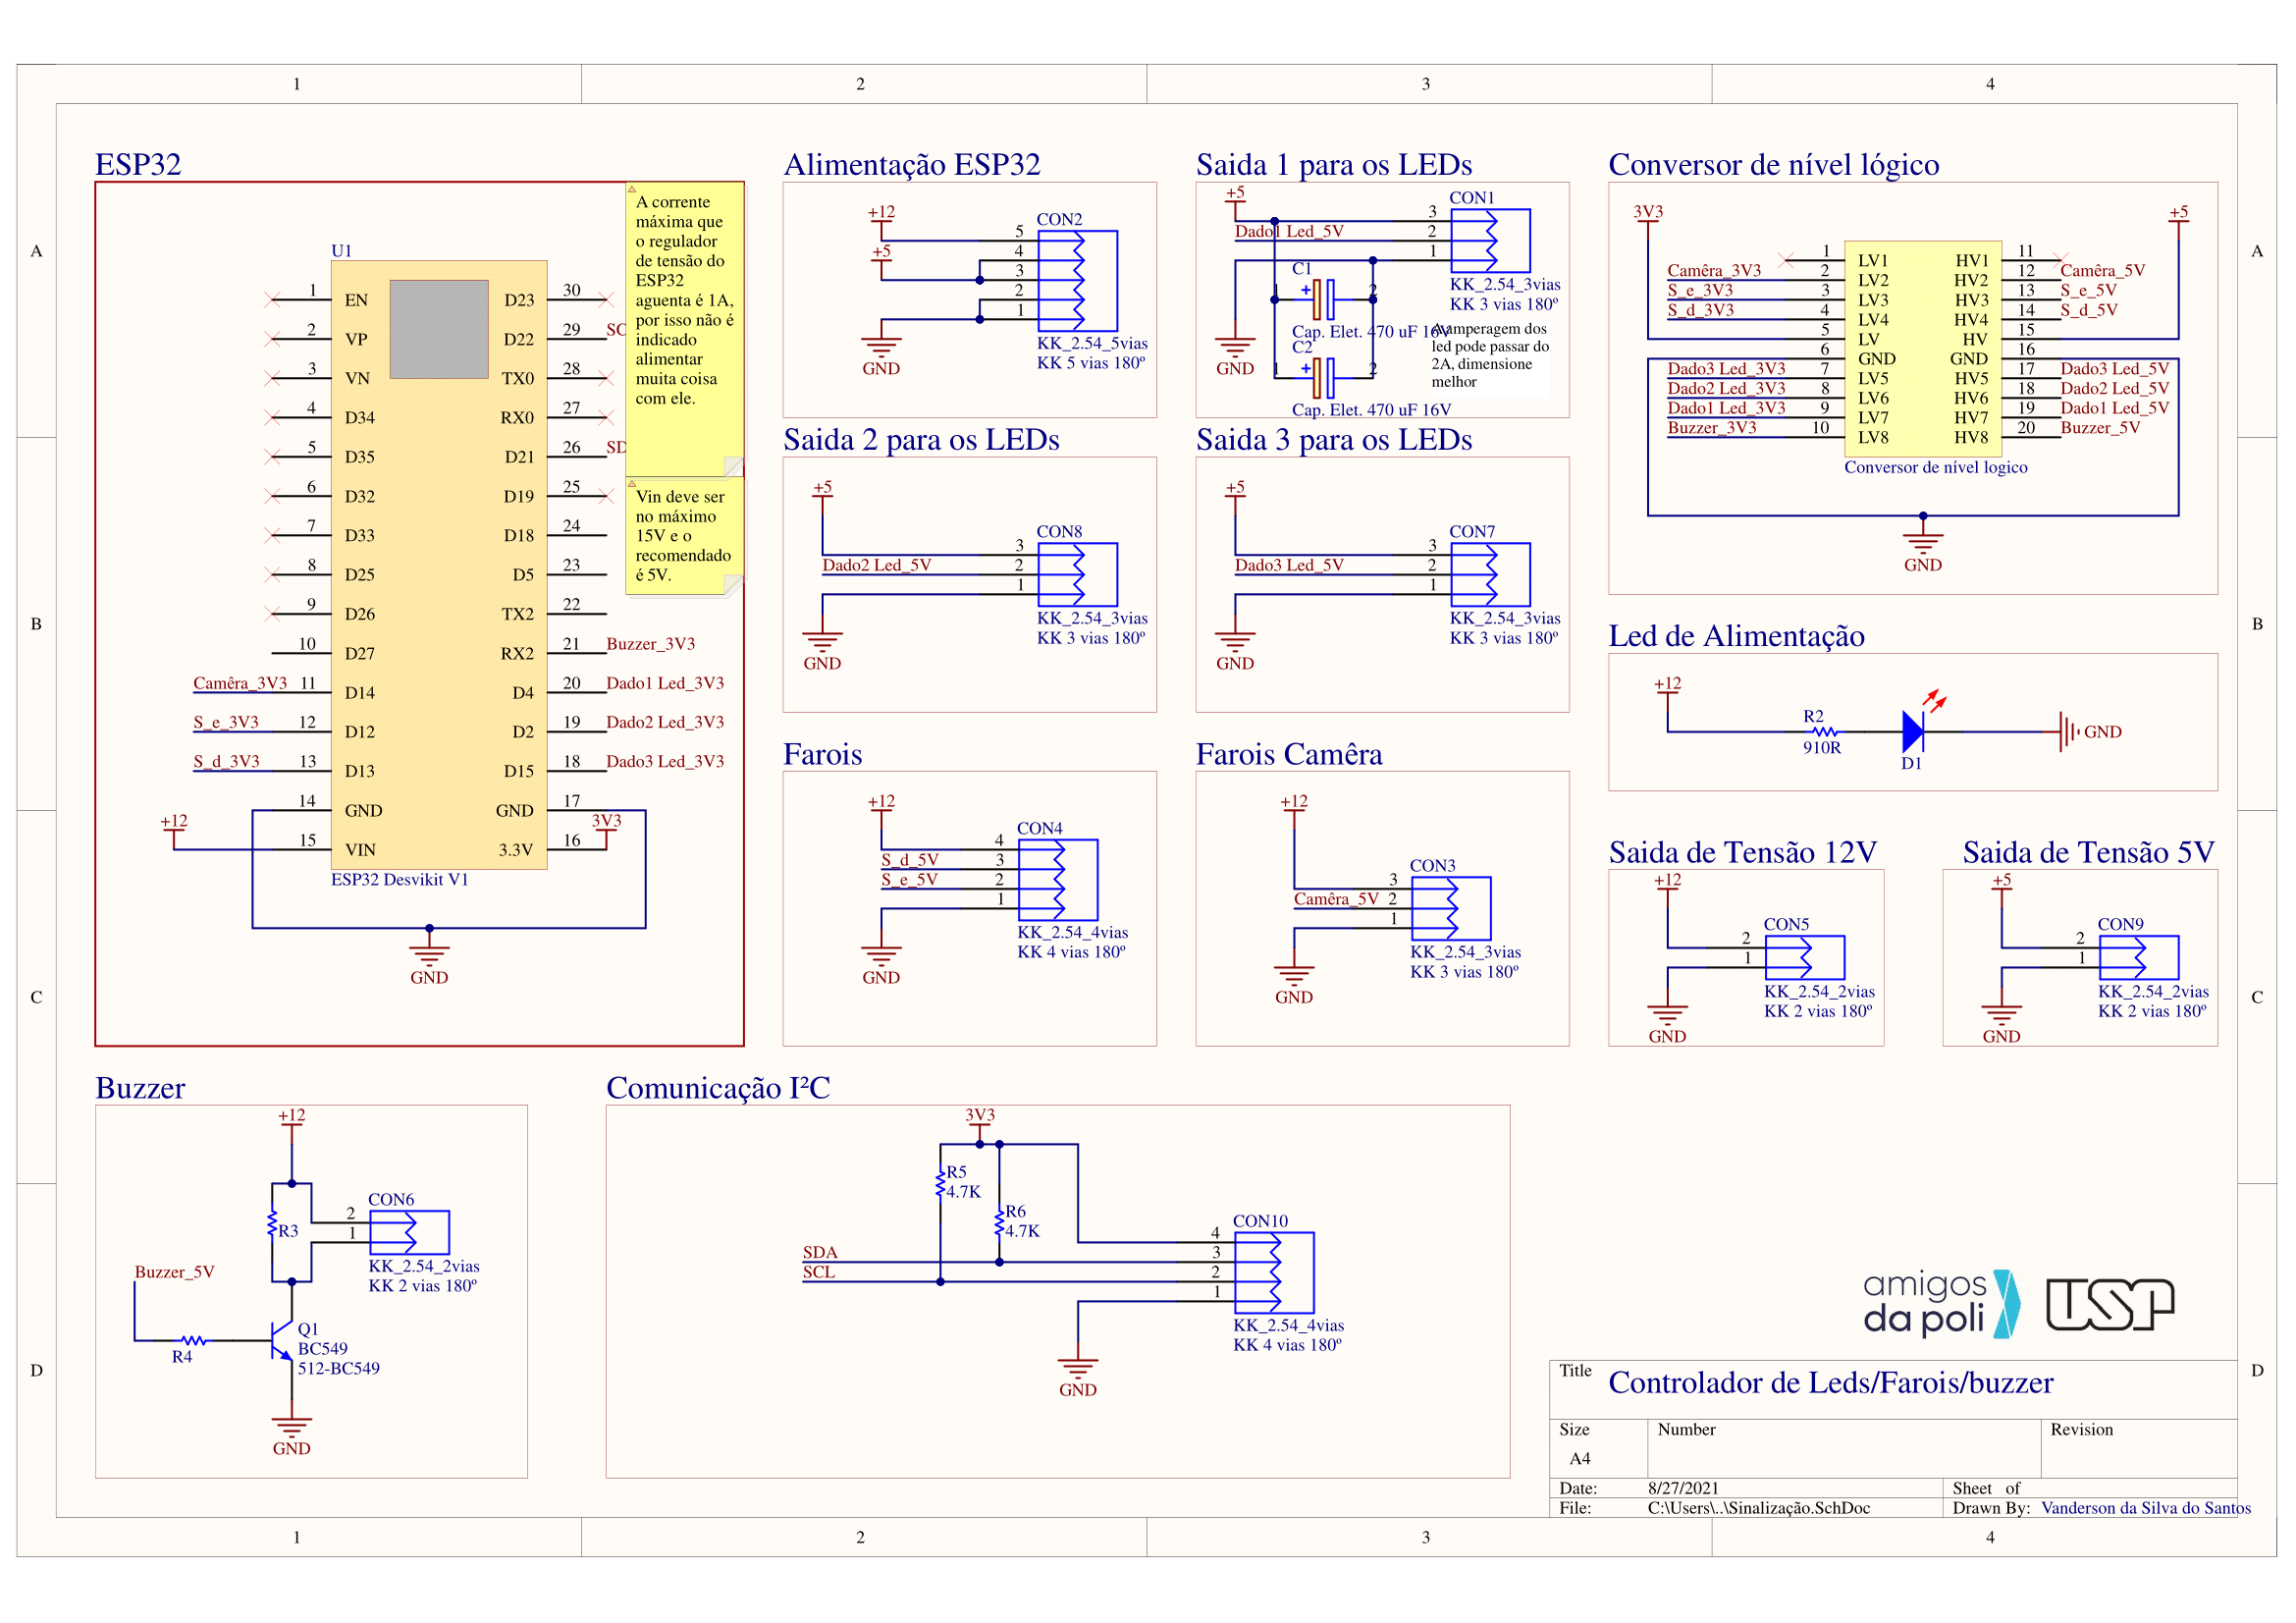
\includegraphics[width=17cm]{modulos/Sinalização-1.png}
    \caption*{Fonte: Elaborado pelo autor no software Altium Design\cite{altium21} }
    \label{Protótipo placa de ## - Esquemático principal}
\end{figure}

\begin{table}[]
\caption{Componentes Utilizados na placa de Sinalização - Protótipo}
\centering
\begin{adjustbox}{width=\columnwidth,center}
\begin{tabular}{|c|c|c|c|c|}
\hline
Component                   & Description                                                    & Designator               & Footprint                   & Quantity \\ \hline
Conversor de   nível logico & Conversor de nível   lógico                                    & U2                       & Conversor de nível   lógico & 1        \\ \hline
Cap. Elet. 470   uF 16V     & Aluminum Organic   Polymer Capacitors 16volts 470uF ESR 10mohm & C1, C2                   & Cap. Elet. 470uF 16V        & 2        \\ \hline
KK\_2.54\_3vias             & Conector KK 2.54mm 3   vias                                    & CON1, CON3, CON7,   CON8 & KK\_3vias\_180º             & 4        \\ \hline
KK\_2.54\_5vias             & Conector KK 2.54mm 5   vias                                    & CON2                     & KK\_5vias\_180°             & 1        \\ \hline
KK\_2.54\_4vias             & Conector KK 2.54mm 4   vias                                    & CON4, CON10              & KK\_4vias\_180°             & 2        \\ \hline
KK\_2.54\_2vias             & Conector KK 2.54mm 2   vias                                    & CON5, CON6, CON9         & KK\_2VIAS\_180º             & 3        \\ \hline
LED 5MM RED                 & LED 5MM RED                                                    & D1                       & LED 5MM RED                 & 1        \\ \hline
BC549                       & TRANS NPN 30V 0.1A   TO-92                                     & Q1                       & TO92                        & 1        \\ \hline
RES 470R 1/4W   CARBON FILM & RES 470R OHM 1/4W 5\%   CARBON FILM                            & R2                       & RES 470R 1/4W CARBON   FILM & 1        \\ \hline
RES 1/4W   CARBON FILM      & RES ? OHM 1/4W 5\%   CARBON FILM                               & R3, R4                   & RES 10K 1/4W CARBON   FILM  & 2        \\ \hline
4.7K                        & RES 4.7K OHM 1/4W 5\%   CARBON FILM                            & R5, R6                   & RES 4.7K 1/4W CARBON   FILM & 2        \\ \hline
microcontrolador            & microcontrolador com   moculo bluethoth e wifi                 & U1                       & ESP32\_Desvikit\_v1         & 1        \\ \hline

\end{tabular}
\end{adjustbox}
\centering
\caption*{Fonte: Elaborado pelo autor}
\label{table:voc}
\end{table}


\paragraph{Printed Circuit board (PCB)}

\begin{figure}[!ht]
    \centering
    \begin{minipage}{0.5\textwidth}
        \centering
        \caption{Protótipo Sinalização - PCB 2D}
        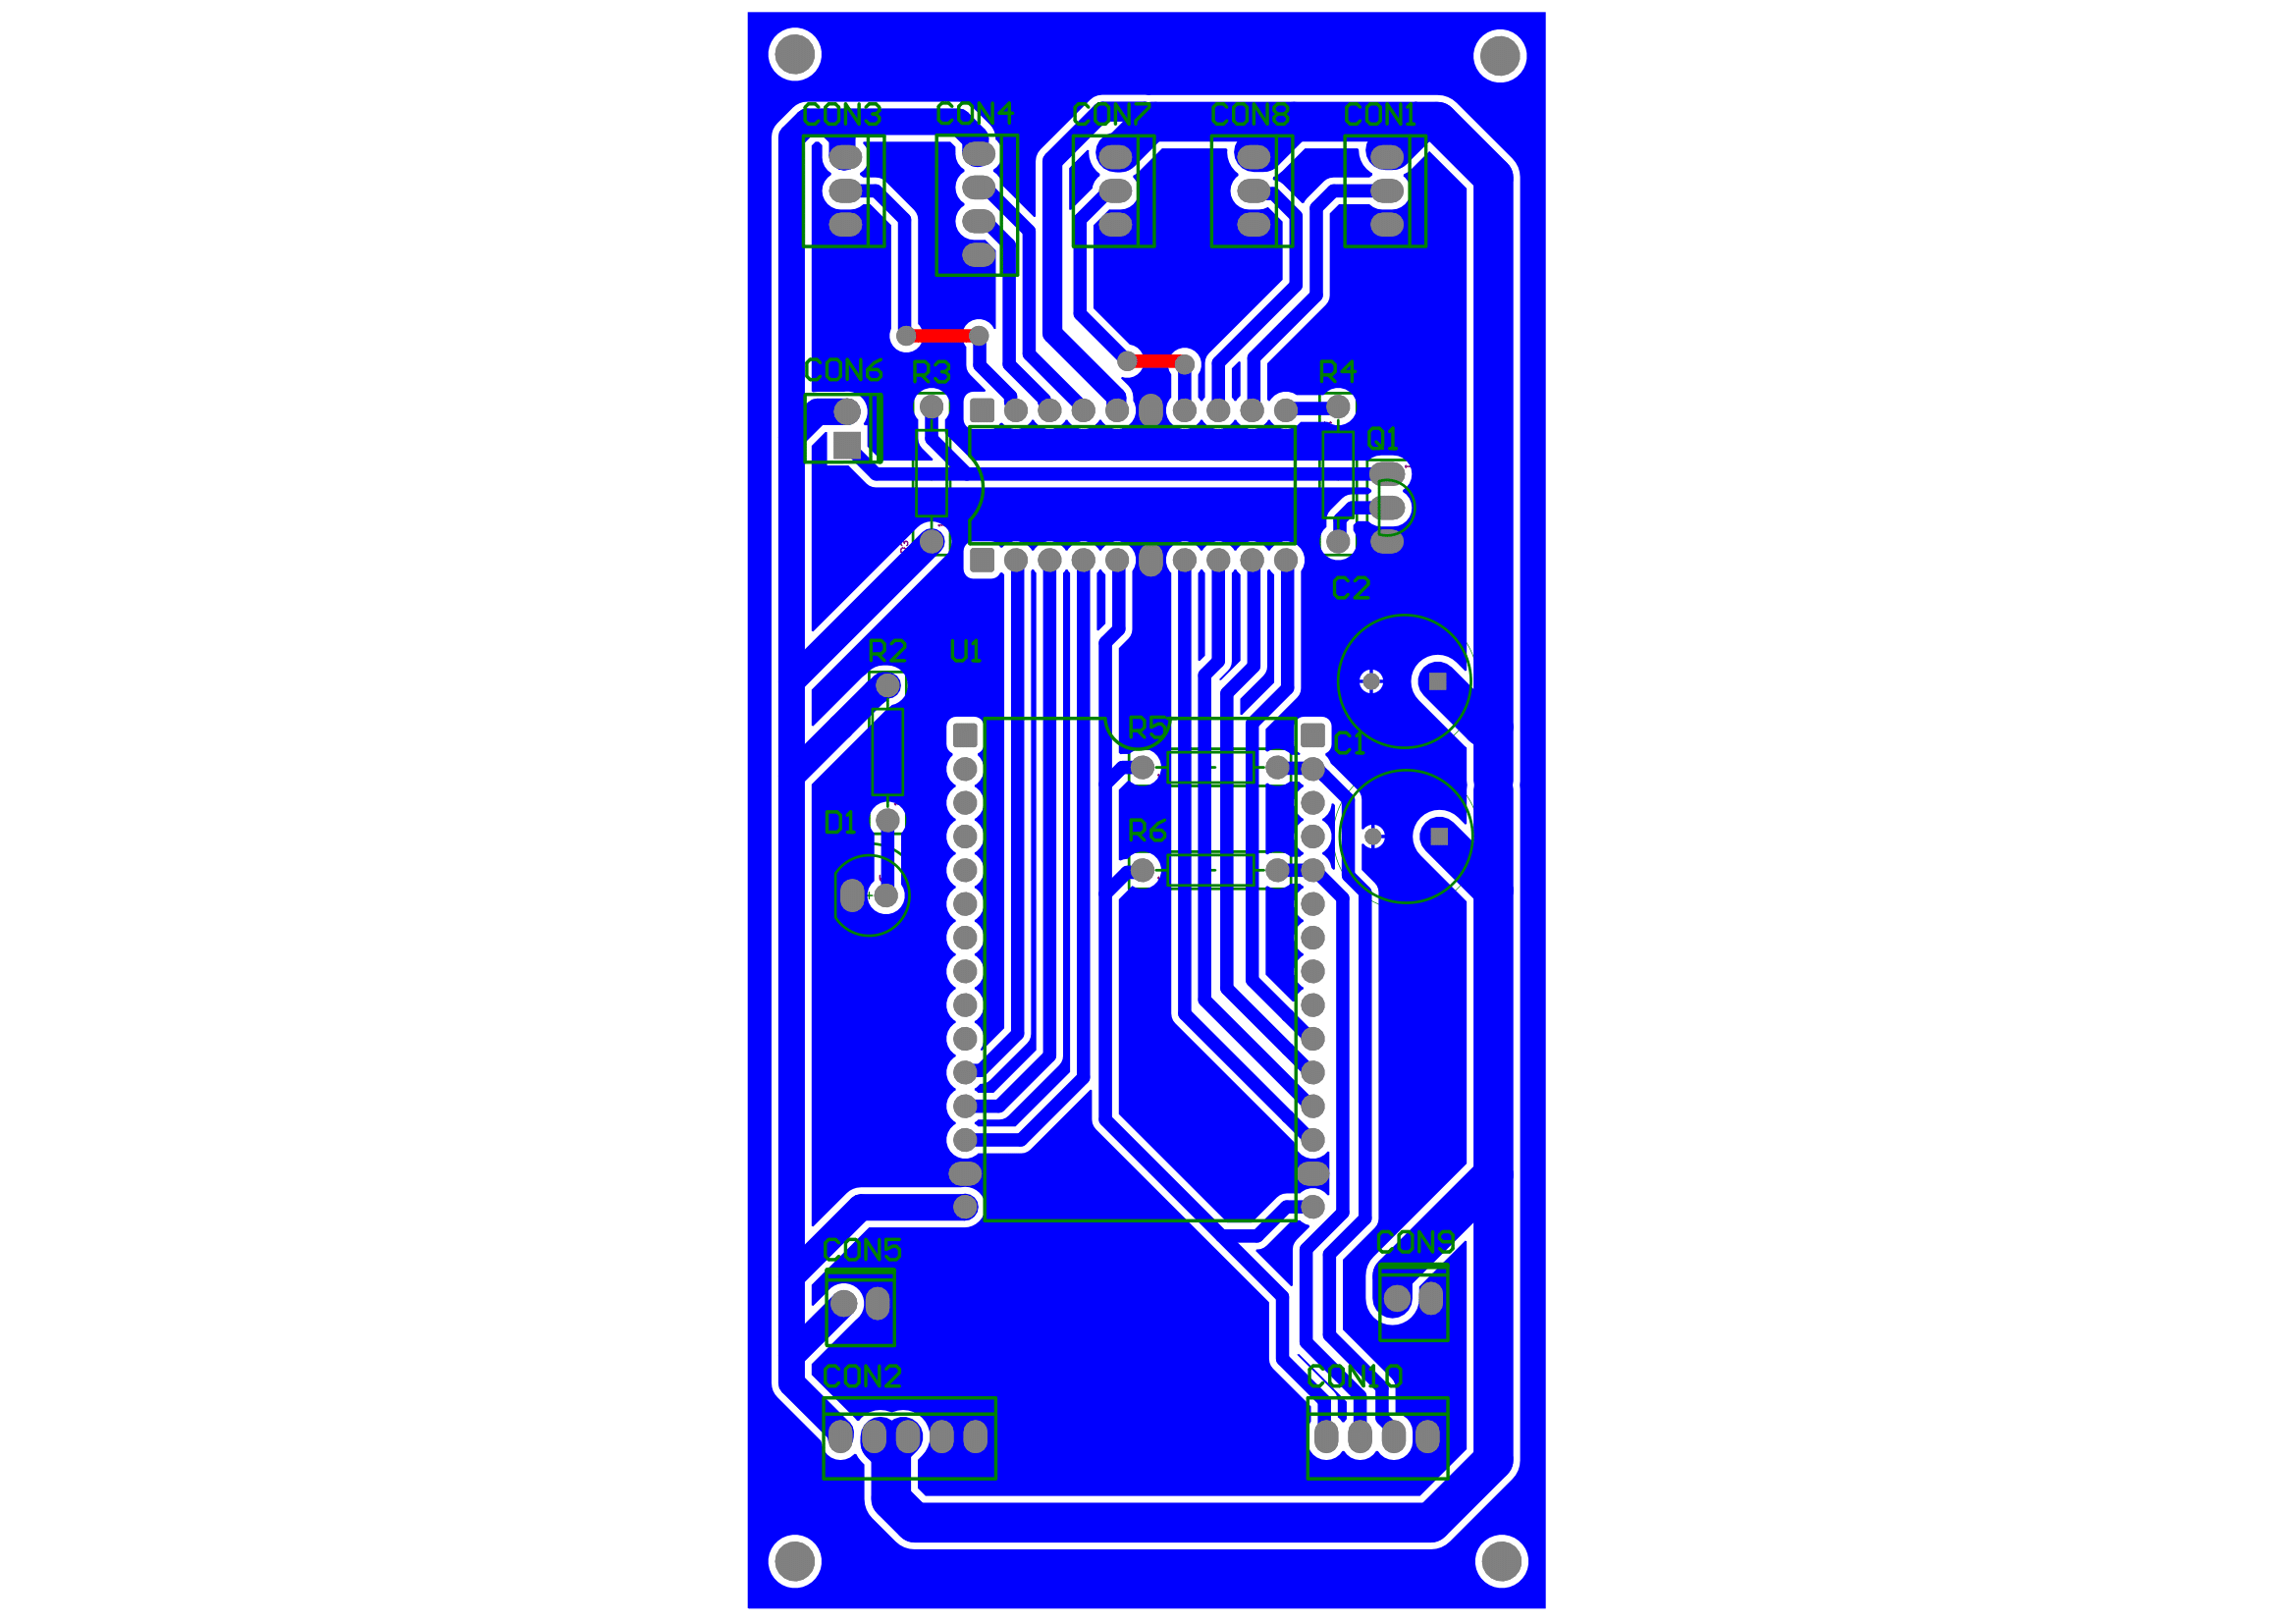
\includegraphics[width=1.03\textwidth]{modulos/Sinalização-2.png} 
        \label{fig:figura1minipg}
    \end{minipage}\hfill
    \begin{minipage}{0.5\textwidth}
        \centering
        \caption{Protótipo Sinalização - PCB 3D }
        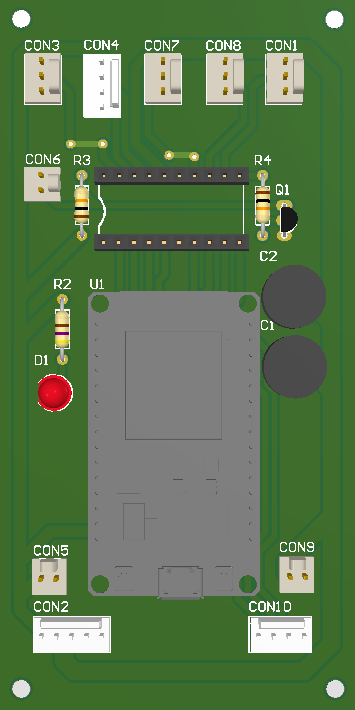
\includegraphics[width=0.4\textwidth]{modulos/Sinalização.png} 
        \label{fig:figura1minipg}
    \end{minipage}\hfill
    
    \caption*{Fonte: Elaborado pelo autor no software Altium Design\cite{altium21} }
    \label{fig:figurasminipg}
\end{figure}

\begin{figure}[!ht]
    \centering
    \begin{minipage}{0.5\textwidth}
        \centering
        \caption{Protótipo Sinalização - Trilhas}
        \includegraphics[width=0.8\textwidth]{example-image-a} 
        \label{fig:figura1minipg}
    \end{minipage}\hfill
    \begin{minipage}{0.5\textwidth}
        \centering
        \caption{Protótipo Sinalização - Completa }
        \includegraphics[width=0.8\textwidth]{example-image-a} 
        \label{fig:figura1minipg}
    \end{minipage}\hfill
    
    \caption*{Fonte: Elaborado pelo autor }
    \label{fig:figurasminipg}
\end{figure}

%================================ SINALIZAÇÂO OfICIAL ========================
\subsubsection{Oficial}

\paragraph{Esquemático}

\begin{figure}[h]
\centering
    \caption{placa de Sinalização - Esquemático principal }
    \centering % para centralizarmos a figura
    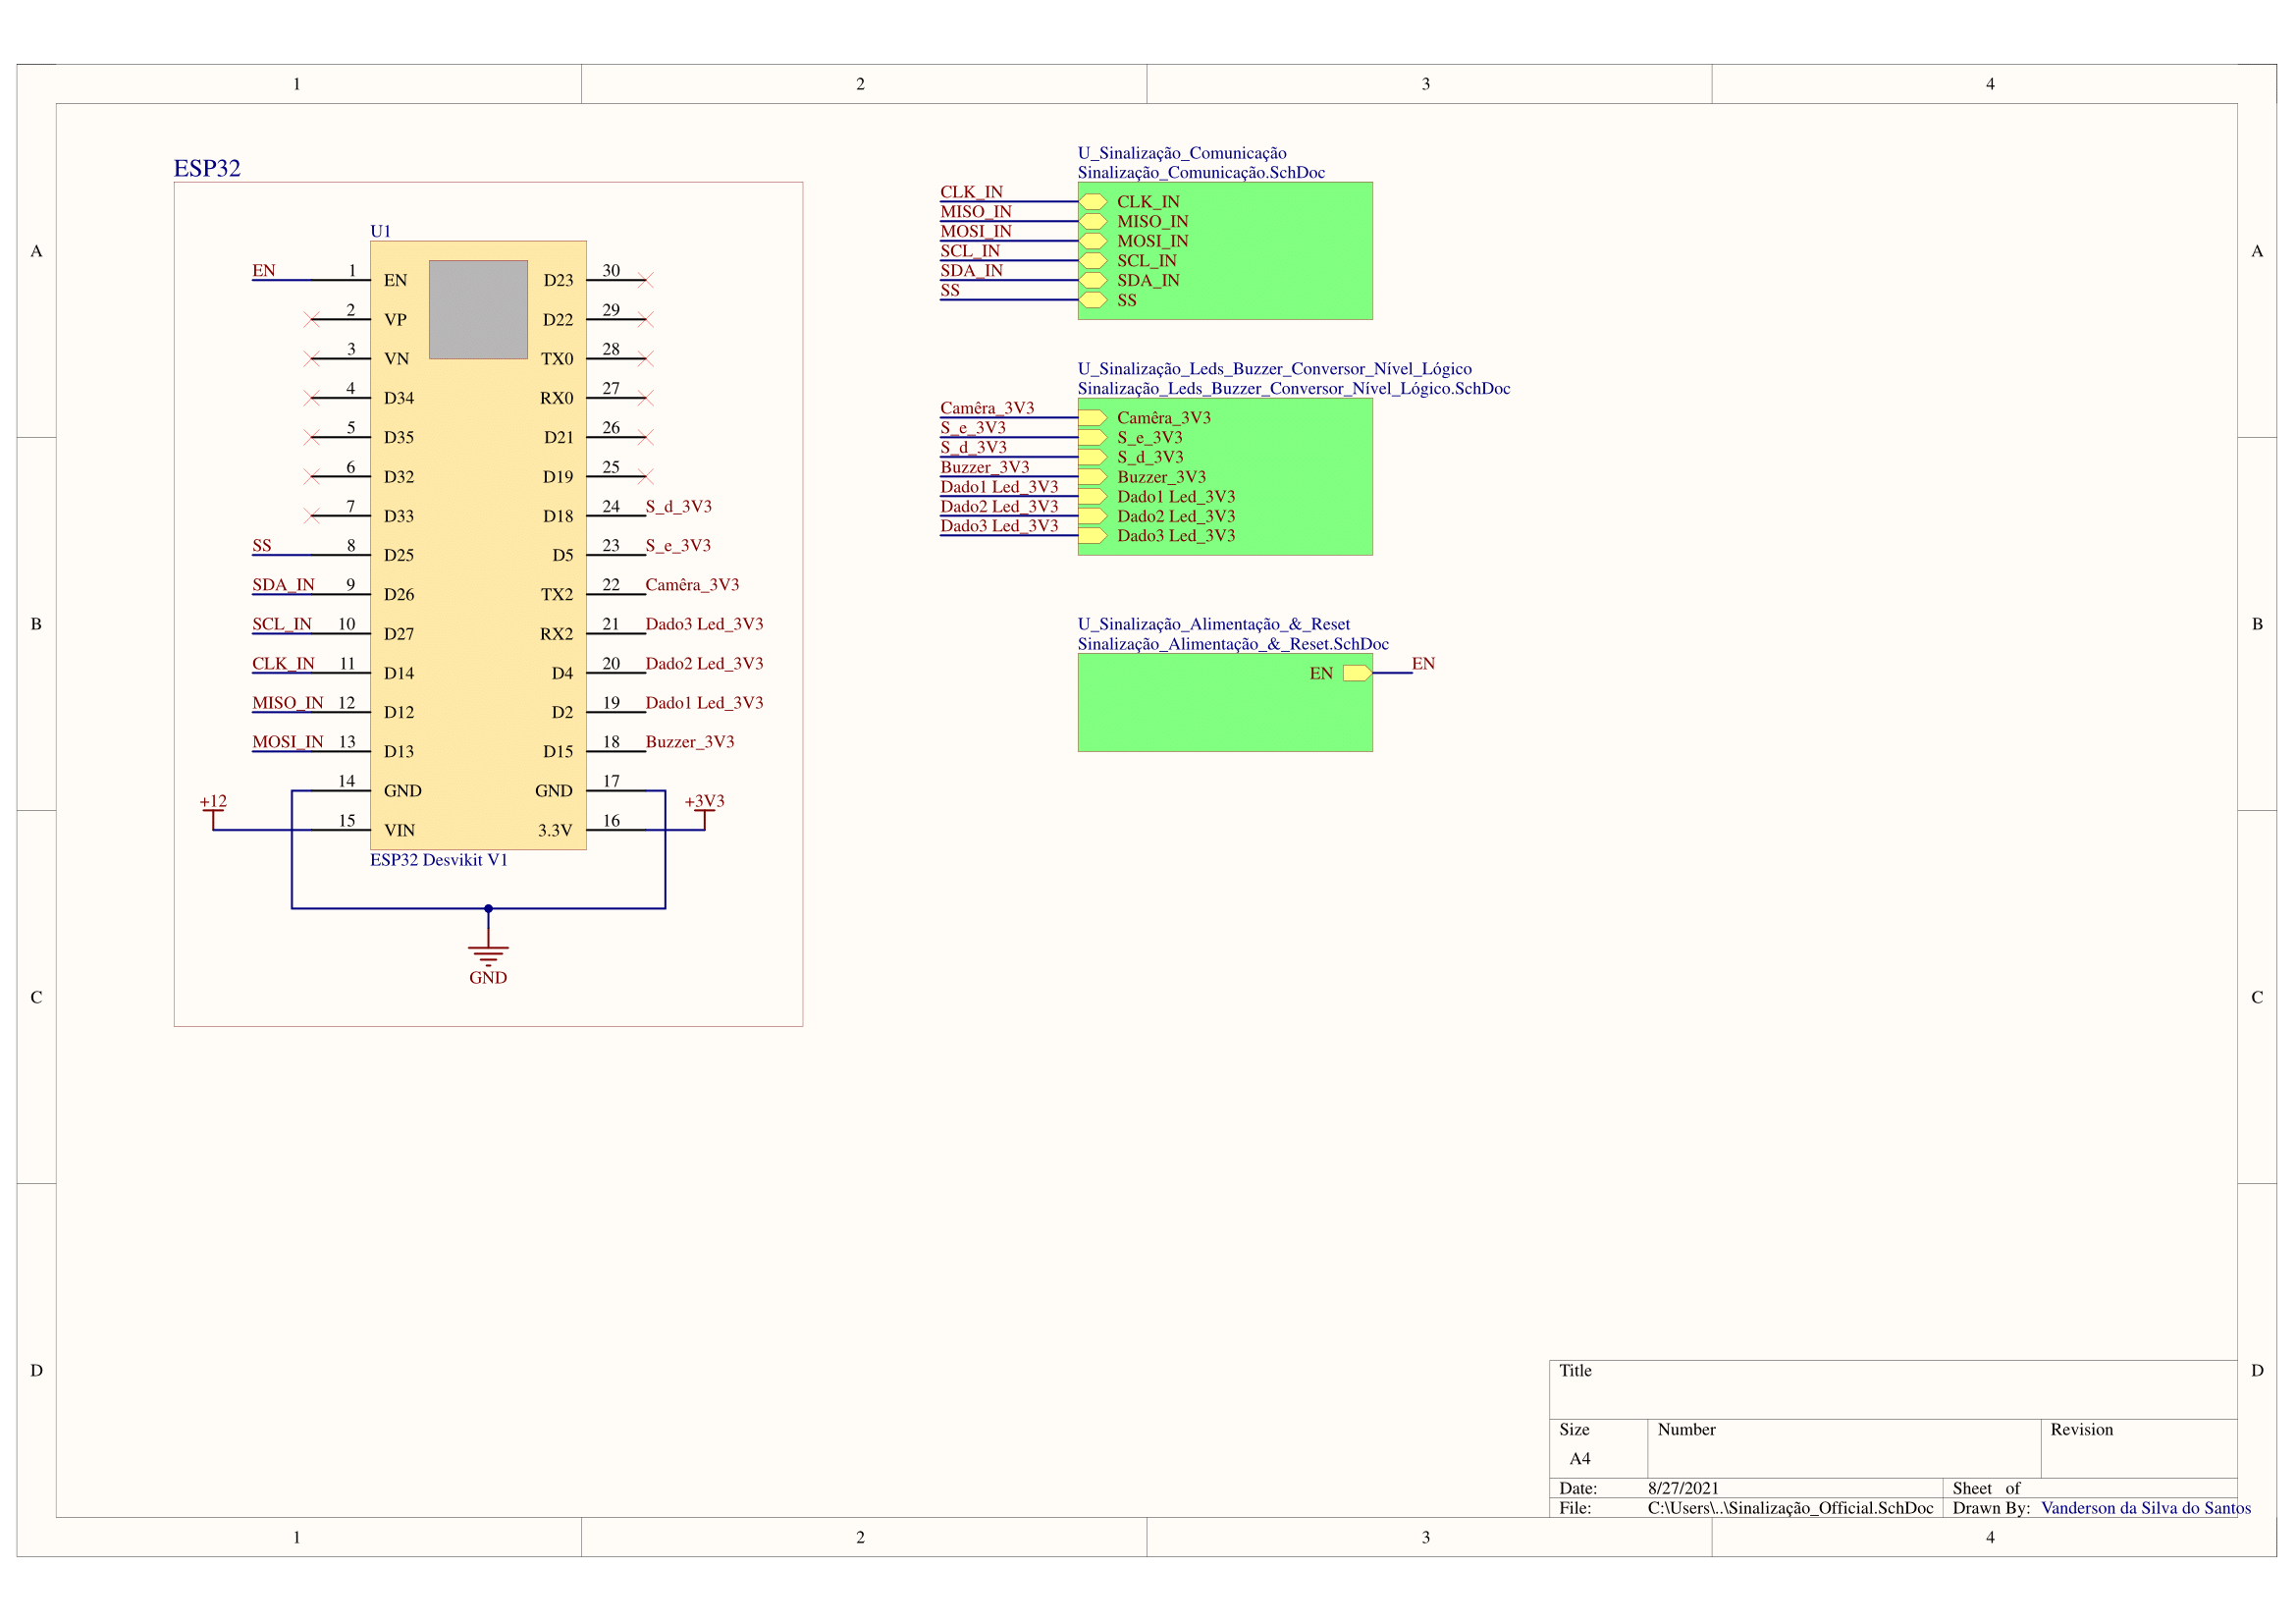
\includegraphics[width=17cm]{modulos/Sinalização_Official-1.png}
    \caption*{Fonte: Elaborado pelo autor no software Altium Design\cite{altium21} }
    \label{Protótipo placa de ## - Esquemático principal}
\end{figure}

\begin{table}[]
\caption{Componentes Utilizados na placa de Sinalização}
\centering
\begin{adjustbox}{width=\columnwidth,center}
\begin{tabular}{|c|c|c|c|c|}
\hline
Comment                   & Description                                  & Designator                & Footprint                 & Quantity \\ \hline
1000uF 50V                & Capacitor Eletrolitico 1000uF 50V            & C1, C2, C3                & CAPPRD500W62D1300H2650    & 3        \\ \hline
KK\_2.54\_5vias           & Conector KK 2.54mm 5 vias                    & CON1                      & KK\_5vias\_180°           & 1        \\ \hline
KK\_2.54\_4vias           & Conector KK 2.54mm 4 vias                    & CON2, CON7                & KK\_4vias\_180°           & 2        \\ \hline
KK\_2.54\_2vias           & Conector KK 2.54mm 2 vias                    & CON3, CON9, CON11, CON12  & KK\_2VIAS\_180º           & 4        \\ \hline
KK\_2.54\_3vias           & Conector KK 2.54mm 3 vias                    & CON4, CON5, CON6, CON8    & KK\_3vias\_180º           & 4        \\ \hline
KK\_2.54\_6vias           & Conector KK 2.54mm 6 vias                    & CON10                     & KK\_6vias\_180°           & 1        \\ \hline
LED 3MM RED               & LED 3MM RED                                  & D1                        & LED RED                   & 1        \\ \hline
Trans BC817               & Transistor BJT NPN BC817-25-7-F              & Q1, Q2                    & SOT96P240X110-3N          & 2        \\ \hline
4K7                       & Resistor                                     & R1, R2                    & RESC3216X60N              & 2        \\ \hline
1K                        & Resistor                                     & R3                        & RESC3216X60N              & 1        \\ \hline
2K2                       & Resistor                                     & R4, R7                    & RESC3216X60N              & 2        \\ \hline
680R                      & Resistor                                     & R5                        & RESC3216X60N              & 1        \\ \hline
Resistor 1206             & Resistor                                     & R6                        & RESC3216X60N              & 1        \\ \hline
microcontrolador          & microcontrolador com moculo bluethoth e wifi & U1                        & ESP32\_Desvikit\_v1       & 1        \\ \hline
Conversor de nível logico & U2                                           & Conversor de nível lógico & Conversor de nível logico &          \\ \hline

\end{tabular}
\end{adjustbox}
\centering
\caption*{Fonte: Elaborado pelo autor}
\label{table:voc}
\end{table}

\paragraph{Printed Circuit board (PCB)}

\begin{figure}[!ht]
    \centering
    \begin{minipage}{0.5\textwidth}
        \centering
        \caption{Sinalização - PCB 2D}
        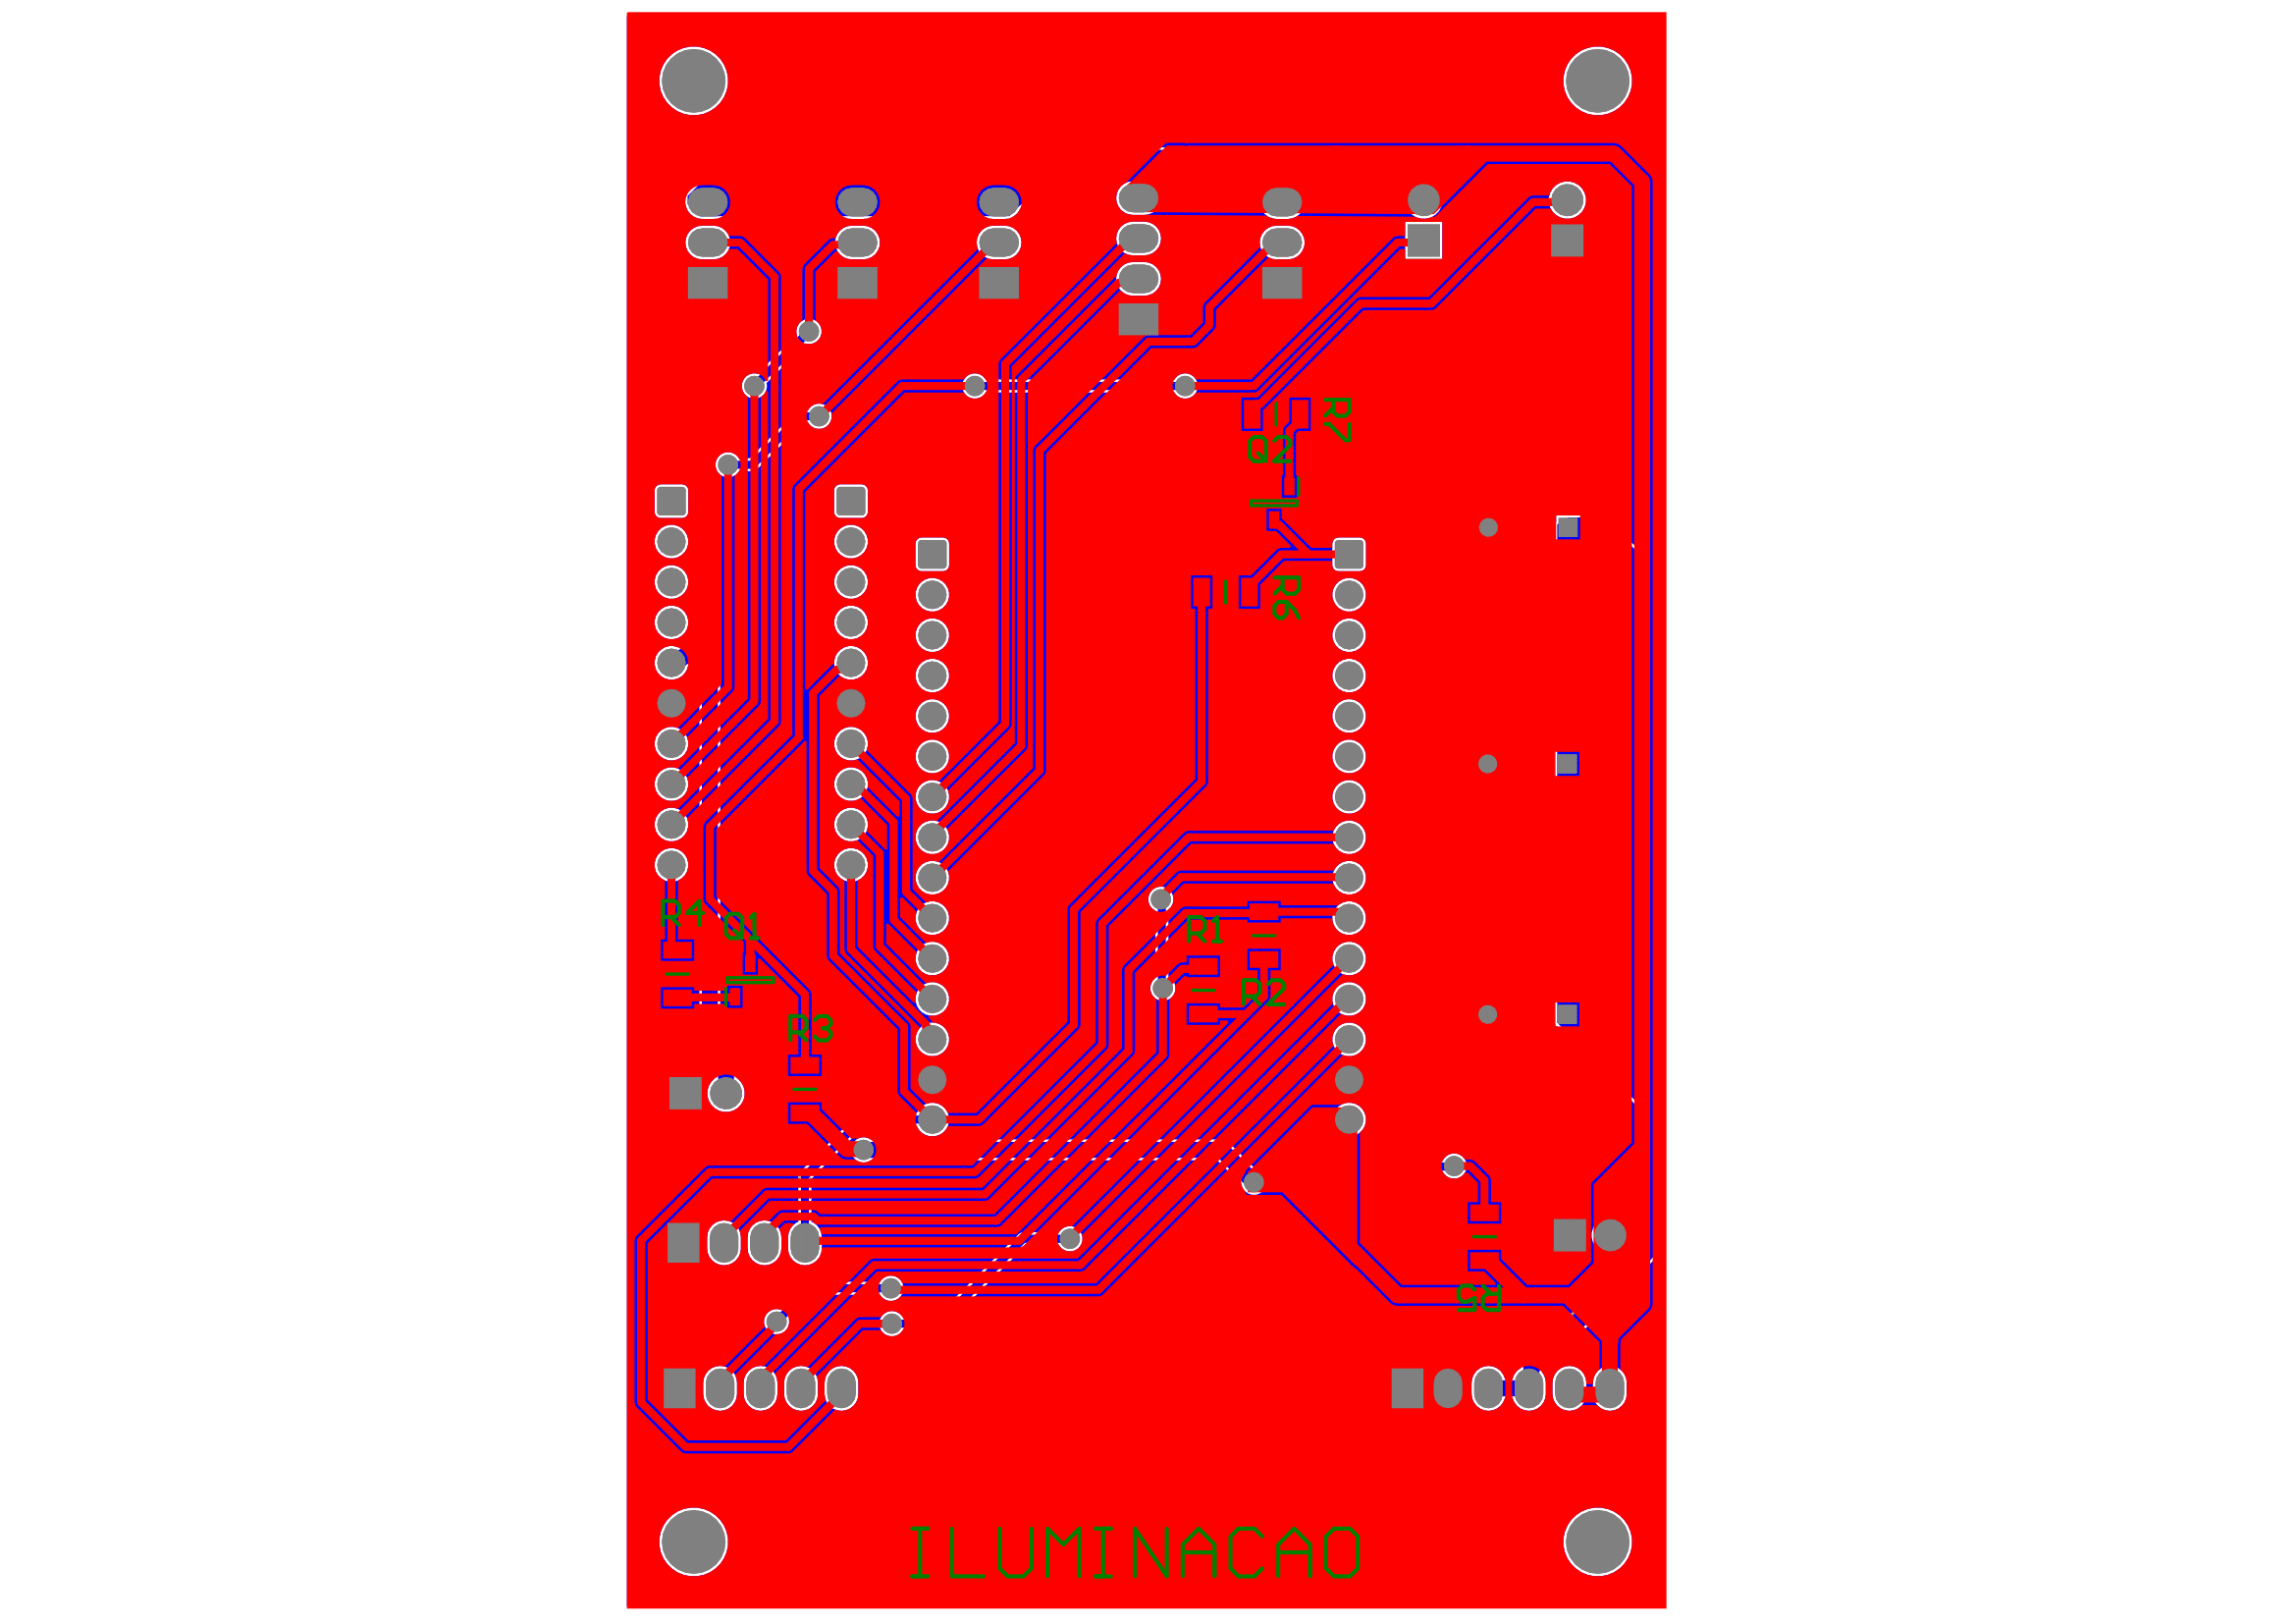
\includegraphics[width=1.03\textwidth]{modulos/Sinalização_Official-5.png} 
        \label{fig:figura1minipg}
    \end{minipage}\hfill
    \begin{minipage}{0.5\textwidth}
        \centering
        \caption{Sinalização - PCB 3D }
        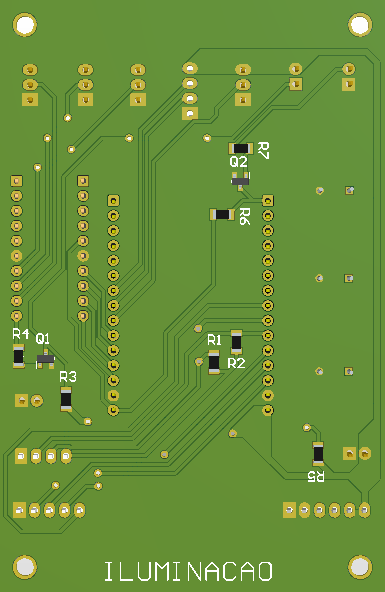
\includegraphics[width=0.4\textwidth]{modulos/Sinalização_Official.png} 
        \label{fig:figura1minipg}
    \end{minipage}\hfill
    
    \caption*{Fonte: Elaborado pelo autor no software Altium Design\cite{altium21} }
    \label{fig:figurasminipg}
\end{figure}

%================================ SINALIZAÇÂO FIRMWARE ========================
\subsection{Firmware}

\end{document}